\subsection{Verarbeitung}
Nachfolgend werden die Methoden beschrieben, welche für die Verarbeitung der generierten Bilder verwendet werden könnten. Je nach Methode könnten diese Funktionen direkt auf den NanoPi implementiert werden. Somit wäre es möglich die Nachverarbeitung zu erweitern und bei sämtlichen Verkehrsteilnehmern diese Funktionen ebenfalls durchzuführen und auszuwerten. Das Resultat daraus wäre ein besserer Feature Vektor, was die Verkehrsverfolgung erleichtern würde.

\subsubsection{GrabCut}
Bei "'GrabCut"' handelt es sich um einen Algorithmus, welcher bereits in OpenCV implementiert ist. Optimal verwendet kann dieser genutzt werden, um automatisch den Hintergrund eines Bildes wegzuschneiden. Bei diesem Algorithmus kann ein Rahmen in das Bild gelegt werden, welcher definiert, was als Hintergrund gewertet werden soll. OpenCV schneidet danach den Rahmen und sämtliche darin enthaltene Ähnlichkeiten aus, bis eine zu grosse Veränderung zwischen den umliegenden Pixeln gefunden wurde. Nachfolgende Abbildung (\fref{bGrabCut}) zeigt ein Beispiel von GrabCut. 

\begin{figure}[H]
  \centering
  \subfigure[Originalbild mit Rahmen]{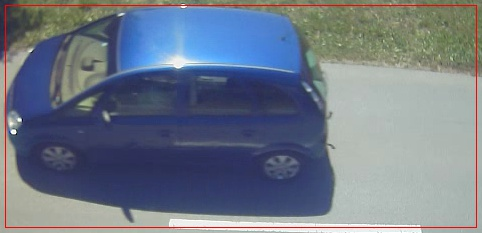
\includegraphics[width=0.49\textwidth]{Testversuche/GrabCut1.jpg}}
  \subfigure[Ergebnis des Algorithmus]{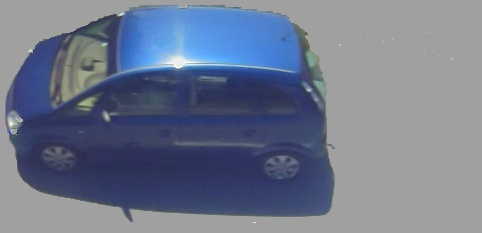
\includegraphics[width=0.49\textwidth]{Testversuche/GrabCut2.jpg}}
  \caption{Beispiel GrabCut}
  \label{bGrabCut}
\end{figure}

Auf dem linken Bild sind das Originalbild und der definierte Rahmen zu sehen, auf dem rechte Bild das Ergebnis dazu. Dem Ergebnis wurde ein grauer Hintergrund hinzugefügt, jedoch kann diese Farbe frei gewählt werden. Je nach Bild, welches verwendet wird, kann GrabCut schlechte bis hervorragende Resultate liefern. Dabei kommt es vor allem darauf an, wie starke Farbveränderungen im Hintergrund vorhanden sind. Bei diesem Algorithmus handelt es sich um eine komplexe Methode, welche selbst auf dem Computer einige Sekunden an Verarbeitungszeit benötigt. \cite{GrabCut}

\subsubsection{Schattenentfernung}
Als die ersten Testaufnahmen durchgeführt wurden, musste festgestellt werden, dass Schatten zu einem grossen Problem führen konnte. Dies trat vor allem dann auf, wenn die Sonne den Schatten des Verkehrsteilnehmers in richtung Kamera projezierte. Dadurch wurde der Bildausschnitt des Verkehrsteilnehmers grösser als er tatsächlich war, was weitere Auswertungen verfälschte. Aus diesem Grund wurde nach Möglichkeiten gesucht, um diesen Schatten zu entfernen, weshalb schlussendlich eine Funktion dafür geschrieben wurde.
Falls ein Schatten vorhanden war, konnte dies am Differenzbild erkannt werden. Dort traten jeweils, waagrecht betrachtet, zwei helle Streifen und dazwischen ein dunkler Abschnitt auf. Auffällig daran ist, dass die Breite der hellen Steifen fast gleich gross waren, was auf die Geschwindigkeit des Fahrzeugs zurückzuführen ist. Der helle Streifen entstand, wenn nur auf einem der beiden Bilder, welche für das Differenzbild zuständig waren, ein Schatten vorhanden war. Der dunkle Abschnitt zwischen den hellen Stellen entstand, wenn auf beiden Eingangsbildern bereits ein Schatten vorlag. Nachfolgende Abbildung (\fref{bBlurRemoveShadow}) zeigt die geschilderte Situation eines Differezbildes mit Schatten.

\begin{figure}[H]
  \centering
  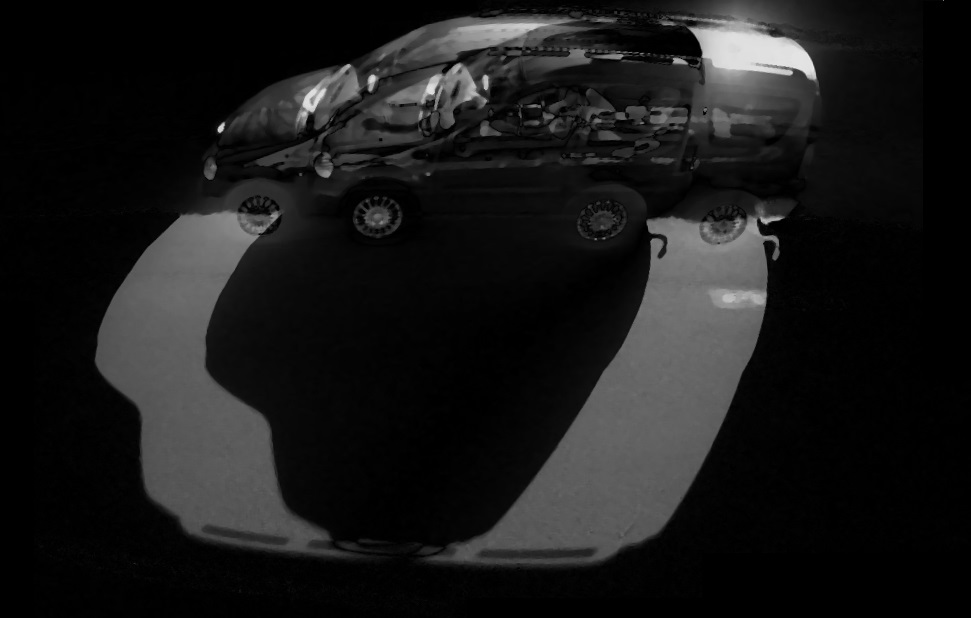
\includegraphics[height=0.3\textheight]{Testversuche/BlurRemoveShadow.jpg} 
  \caption{Differenzbild zur Demonstration des Schattens}
  \label{bBlurRemoveShadow}
\end{figure} 

Beim Algorithmus der Funktion wird jeweils 